\chapter{Evaluation}\markright{Chapter 5: Evaluation}\label{sec:evaluation} 
In order to demonstrate the effectiveness of our scheme, we evaluate Accuracy of each defense method compared to the previous scheme.
Accuracy is calculated as:
\begin{equation}
  \mathrm{Accuracy} = \frac{\mathrm{TP}+\mathrm{TN}}{\mathrm{TP} + \mathrm{TN} + \mathrm{FP} + \mathrm{FN}}, 
\end{equation}
where TP, TN, FP, and FN denote the number of True Positive (malwares are regarded as malwares), True Negative (benign files are regarded as benign ones), False Positive (benign files are regarded as malwares), and False Negative (malwares are regarded as benign files), respectively.  

\section{Simulaion parameters}
\tablename~\ref{tab:simulation_parameters} shows our simulation parameters.  
\begin{table}[p]
	\begin{center}
		\caption{Simulation Parameters}
		\label{tab:simulation_parameters} 
		\begin{tabular}{|c|c|} \hline
			The name of parameters & Value\\ \hline \hline
			Benign files & Ubuntu 16.04.3\cite{ubuntu}\\ \hline
			\multirow{2}{*}{\hfill Malwares  \hfill} & IoTPOT\cite{iotpot} \\ 
																							 & VirusTotal\cite{virustotal}\\ \hline
			The number of benign files  & 1,442 \\  \hline
			The number of malwares  &  7,263 \\ \hline
			The AM attack method & White-box \cite{yamafumi} \\ \hline
			\multirow{2}{*}{\hfill The packing tools for OM  \hfill} & UPX\cite{upx} \\ & kiteshield\cite{kiteshield} \\ \hline
			The number of samples  & \multirow{2}{*}{\hfill 800 \hfill} \\  
			in AM-resiliency evaluation & \\ \hline 
			The number of samples  & \multirow{2}{*}{\hfill 1000 \hfill} \\  
			in OM-resiliency evaluation & \\ \hline 
		\end{tabular}
	\end{center}
\end{table} 


We use the benign files from Ubuntu system files \cite{ubuntu} as the begin files.
Meanwhile, malwares are collected from IoTPOT \cite{iotpot} and VirusTotal \cite{virustotal} which is a repository of malware samples for security researchers.
In order to use those samples as inputs for CNN, we convert each sample to the correponding GSI by following the same procedures implemented in \cite{previous}.
In particular, a binary can be reformatted to a sequence whose elements are 8-bit strings.
Then, each string can be converted to a decimal number which can be seen as the value of a one-channel pixel.
After that, we rescale the GSIs to the size of 64*64 such that they can be input to the CNN.
In particular, manipulated malwares for each attack are created with an adversarial technique implemented in \cite{ae} and two packing tools \cite{upx, kiteshield} shown in \tablename~\ref{tab:simulation_parameters}.

In the case of AM-resiliency evaluation, we apply a white-box method as a adversarial technique for AM, where an the adversary knows the training data and the structure of the CNN model since it is currently the mainstream in this reserch field.

In the case of OM-resiliency evaluation, we use two packing tools, called UPX \cite{upx} and kiteshield \cite{kiteshield}, in order for malwares to be obfuscated.
The UPX is a tool which is often utilized mainly for software compression purposes and, according to \cite{pack_research}, the use of it is confirmed in more than 50\% of obfuscated malwares. 
Meanwhile, the kiteshield is a tool which is often utilized mainly for the purpose of encrypting softwares.
Especially, in this evaluation, we prepare three dataset on the basis of which tools to be used for their obfuscation in order to show the versatility in that our scheme is independent of the packing tools.
Two datasets of the three are composed of malwares obfuscated by each packing tooks, UPX and kiteshield, and the other are mixed malwares from those datasets. 

In the evaluation in respective evaluation, some of the samples from total manipulated malwares, 800 samples in AM attack scenario and 1000 samples in OM attack scenario, are picked randomly, then utilized as inputs in order to keep balance between the number of malwares and that of benign ones.

\section{Evaluation of the invalidating adversarial byte sequences against AM attack}


\section{Evaluation of the method with 1D convolutional filters against OM attack}
\begin{table}[p]
  \begin{center}
    \vspace{-8pt} 
    \caption{The datasets used for the OM-resiliency evaluation}
    \label{tab:schemes} 
    % \vspace{-8pt} 
    % \hspace{-10pt} 
    \begin{tabular}{|c|c|c|} \hline
      \multirow{2}{*}{\hfill  \hfill} & \multicolumn{2}{c|}{Accuracy}  \\ \cline{2-3} 
					     & Prev. (2D filters) & Prop. (1D filters) \\ \hline \hline
      UPX & 94.8\% & 96.2\% \\ \cline{1-3} 
      kiteshield & 85.0\% & 87.8\% \\ \cline{1-3} 
      mix & 86.2\% & 90.0\% \\ \cline{1-3} 
  \end{tabular}
  \end{center}
\end{table}



\begin{table}[p]
  \begin{center}
    \caption{\Our evaluation result}
    \label{tab:result} 
    \begin{tabular}{|c|c|c|c|} \hline
      Scheme & Accuracy(\%) & TPR (\%)& FPR (\%) \\ \hline \hline
      % Prop.1 & 89.0 & 84.7 & 7.83  \\ \hline
      \Our scheme & 89.0 & 84.7 & 7.83  \\ \hline
      Previous Scheme & 86.6 & 80.2 & 8.58  \\ \hline 
      SSL certificate based scheme  & 86.6 & 83.2 & 10.1 \\ \hline
      Permission based features & 86.6 & 76.2 & 5.69  \\ \hline
      \Our scheme  & \multirow{2}{*}{89.9} & \multirow{2}{*}{86.3} & \multirow{2}{*}{7.40} \\ 
       \& previous scheme  &  &  &  \\ \hline 
      % SSL certificate based scheme & \multirow{2}{*}{89.5} & \multirow{2}{*}{82.9} & \multirow{2}{*}{7.40} \\ 
       % \& previous scheme  &  &  &  \\ \hline
    \end{tabular}
  \end{center}
\end{table} 
\afterpage{\clearpage}
\newpage

\figurename~\ref{fig:important_prev_feature} shows the average values of the top 5 important previous features of the malwares detected only by \our scheme.
\begin{figure}[p]
	% \centering
	% \includegraphics[scale=0.35]{./figure/important_prev_f.pdf}
	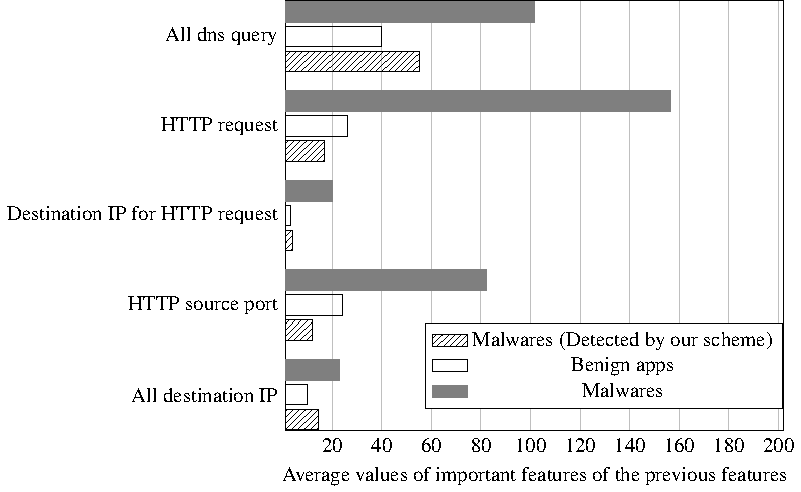
\includegraphics[scale=1.0, bb=10 10 250 250]{./figures/important_prev_f_tikz.pdf}
  \caption{Average values of top 5 important previous features} 
  \label{fig:important_prev_feature}
\end{figure}

As shown in \figurename~\ref{fig:important_prev_feature}, these features of the malwares detected by \our scheme are similar to the benign ones.
\afterpage{\clearpage}
\newpage


\afterpage{\clearpage}
\newpage


